%
% methods_server_side.tex
%

The server-side architecture relies on one primary abstraction for datapaths, a standardized format for different data “channels,” and a configuration file.  These abstractions are utilized by a single server-side driver layer to handle client data requests.  The driver will use these abstractions to solve the issues of data scaling, data sources, and dataset filtering and security.  Specifically, the driver should capture client requests and use a configuration file parameter to validate the request.  If a client requests a dataset that isn’t available or the client isn’t permitted to access, the configuration file validation should filter out that dataset from the request. Next, the driver should use datapaths to acquire data across various data channels and form a response to the client.  This data acquisition process is visualized in Figure \ref{fig:server-side-request} with a concrete examle of a request's processing flow.  To equate this system to an MVC (Model-View-Controller) architecture: the driver is the server’s controller, the datapaths are the controller’s interface to the model, the models are represented by data channels, and the client is the view.  Data channels are a construct available within data paths to represent different models or data sources that are accessed simultaneously and transparently to the driver.  Finally, the configuration file(s) allow the developer freedom to govern dataset availability. \par
  \begin{figure}
    \centering
    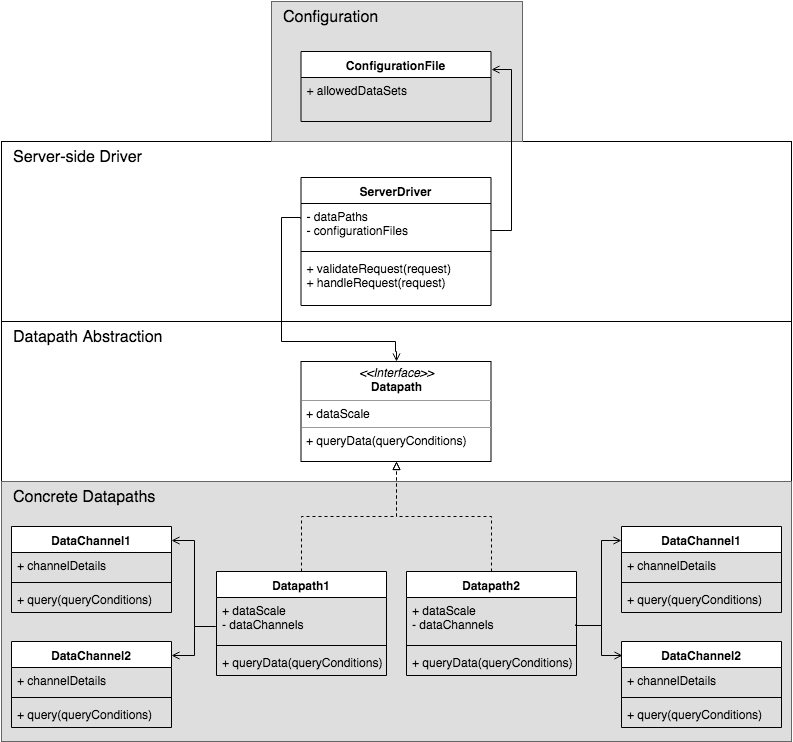
\includegraphics[width=6in]{images/ServerSideClassDiagram.png}
    \caption{Server-Side Class Diagram}
    \label{fig:server-side-class}
 \end{figure}
 \begin{figure}
   \centering
   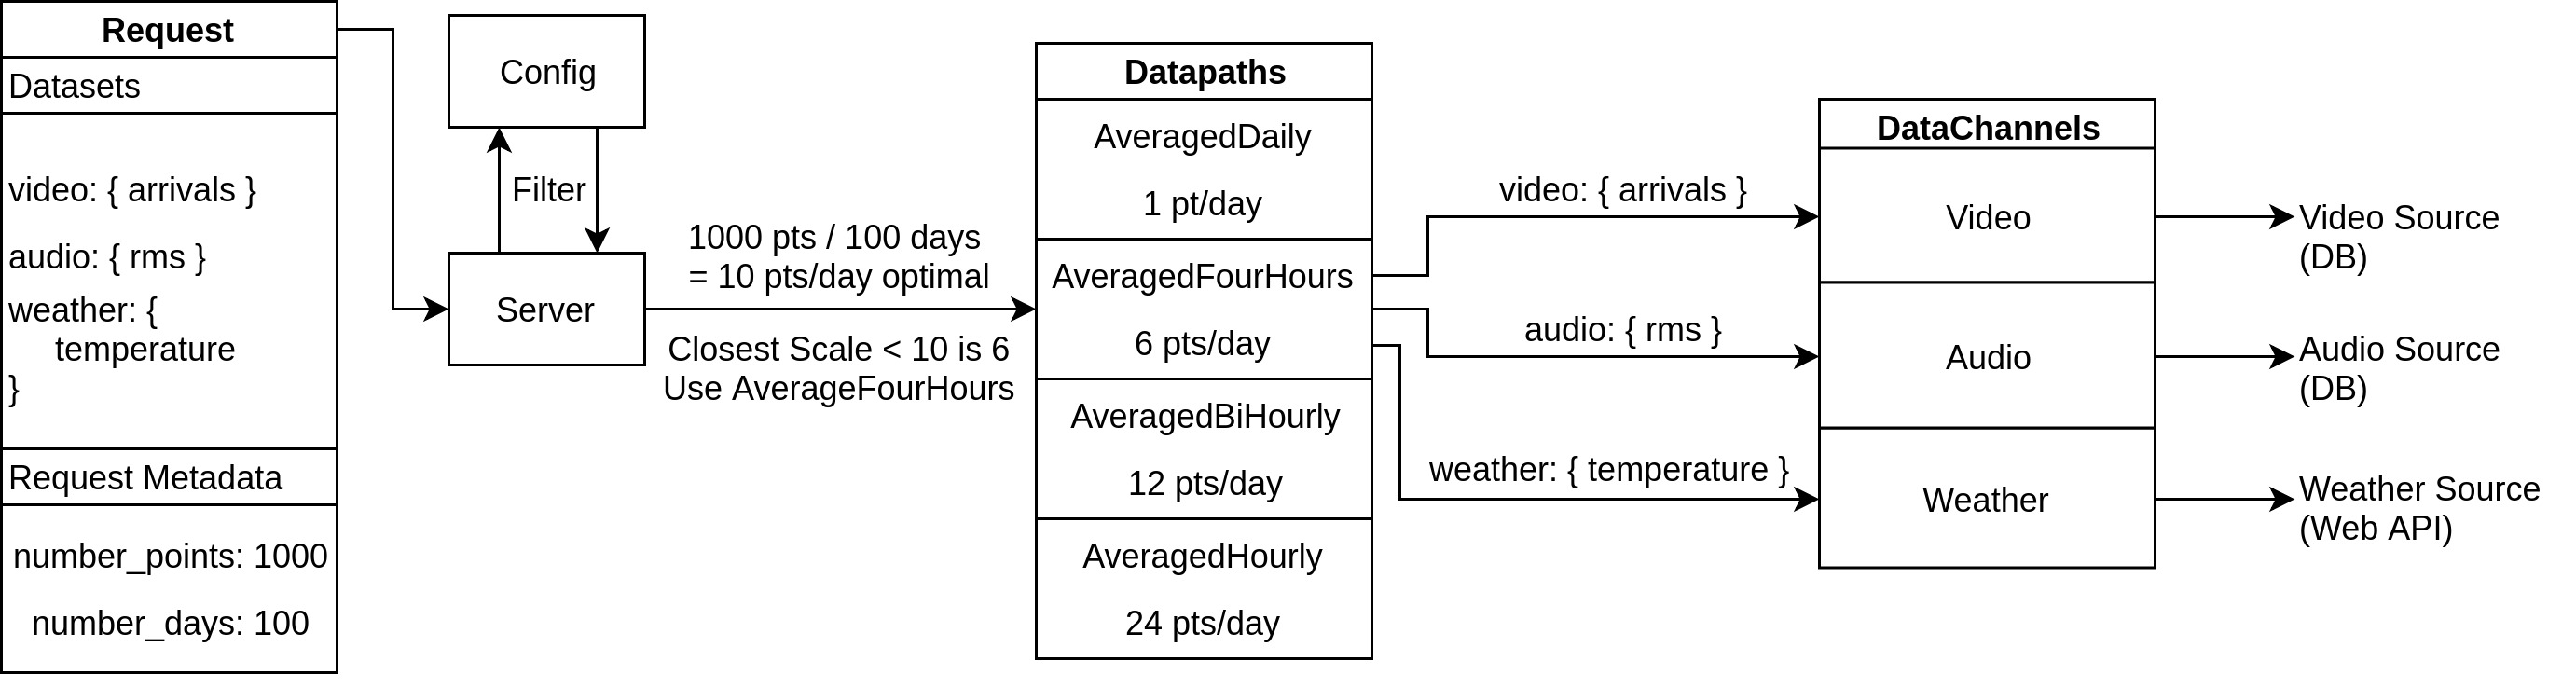
\includegraphics[width=6in]{images/DatapathDataChannelExample.jpg}
   \caption{Request Process Flow}
   \centering{The server receives a request for 1000 data points across 100 days.  It filters this request through the configuration file, selects the optimal datapath by data scale, and queries from that datapath.  The datapath splits the request by channel and queries the data channels, for example \textit{video: \{ arrivals \}} indicates the arrivals dataset should be quired from the video data channel.}
   \label{fig:server-side-request}
 \end{figure}
The server-side implementation is separated into two key segments: driver code and modular code.  This division can be seen in Figure \ref{fig:server-side-class}.  In the figure, all driver code is found within white blocks and all modular code can be found within grey blocks.  The goal of modular segments is to encapsulate the primary modes of change for the server-side.  This means that the developer only needs to define driver code once, but may revise, add, or remove modular elements as required. The driver is responsible for processing client requests, filtering them using configuration files, and responding to requests using data from datapaths.  Within this system, data scaling and data sources are encapsulated within datapaths and dataset filters are encapsulated within the configuration file layer. \par

\subsection{Datapaths}
Datapaths are the primary server-side abstraction built specifically to solve the issues of data scaling and data sources.  The goal of a given datapath is to encapsulate data accesses and scaling within a common interface such that the driver can dynamically interact with different datapaths.  The developer can define multiple datapaths by extending the datapath interface.  The datapath interface requires the developer to define a field which informs the driver of the datapath’s data scale and a function to query data given query conditions as input.  The query function should handle all data acquisition from one or more data channels and any data aggregation.  The dataScale field should export some common metric to measure scale such as items returned per unit, for example the number of data points returned per day.  The driver will import multiple datapaths and use their dataScales to determine which to use when handling a request. \par
When the developer implements a concrete datapath, they can handle data scaling as desired.  For example, a certain dataset may contain one thousand points and include a datapath to scale this data to only one hundred points.  This datapath could aggregate the data in groups of ten by taking the minimum, maximum, average, median, etc.  The proper aggregation method will be depend on the data and the desired result.  This is the reason behind the datapath system, the developer is free to aggregate data sets to different scales, and using different methods of aggregation. \par
Concerning concrete implementation of this architectural element, Beestream implements datapaths by making use of JavaScript’s module system.  Each datapath is defined as a module that exports a query function and a dataScale value.  All datapaths are placed in a single folder within the server-side project code.  The server’s driver code dynamically imports all files within the datapaths folder and will save any file that matches the datapath interface to a list.  The driver will validate that each imported file exports a query function and a dataScale value before saving it to a list of usable datapaths.  This system behaves almost identically to an object-oriented interface and concrete class system, only the driver must enforce the interface explicitly.  Whenever the server receives a request, it will find the dataScale that will provide a number of points closest to the desired number of points.  It will call this datapath’s query function to access data to be delivered to the client.  Beestream’s datapaths provide different data scaling levels using multiple MongoDB aggregate views.  Different views aggregate time-series data hourly, bi-hourly, and daily.  These MongoDB views perform better than querying the full dataset and aggregating in JavaScript within the datapath. \par

\subsection{Data Channels}
Datapaths offer the driver a common interface to access different data sources.  Each datapath can draw data from numerous different data channels.  A data channel represents a single data source.  Much like a television or radio channel allows an individual to access different data through the same medium, the datapath can query from multiple channels to get different data from different datasets through the same interface.  The primary goal of data channels is to separate the driver from various data sources.  This is accomplished by allowing the driver to ask for datasets from a channel by nesting the dataset within a JSON object for that chanel.  For example, when the driver is asked for a temperature value which exists on the weather data source, it will request “weather: {temperature}”.  The datapath will interpret this as a request to query for the temperature dataset from the weather channel as visualized in Figure Figure \ref{fig:server-side-request}.  When the driver receives a result from the dataset, it will receive “temperature” as desired without the knowledge that the dataset had to be queried from a different data source. \par
Data channels reside within modular code, so they are not strictly enforced in the architecture.  The primary goal of data channels is to suggest that different data sources be encapsulated for reuse and feature a common interface.  Datapaths are a suggested feature, but ultimately the developer who defines various datapaths should identify their different data sources and encapsulate them as is appropriate.  If the same data sources are used in multiple places, then they should likely be encapsulated and reused.  If a data source is only used once, then it likely doesn’t need encapsulation.  Data sources’ interfaces can also vary greatly, encompassing various database solutions and web APIs.  As a result, it would be difficult to architecturally require a single interface for data sources, so this choice is left up to the developer writing the datapaths.  Code reuse and modularity is still encouraged. \par
In Beestream’s concrete implementation of data channels, data channels are not expressly abstracted.  Beestream only uses three MongoDB collections as data sources, so they are directly queried using the same interfacing package, called Mongoose.  All queries are executed in parallel using the Async package.  If the project wanted to include data from a web API, that would likely be added through an abstraction to create the same interface as a Mongoose collection following the suggestion that data channels should share an interface if possible. \par

\subsection{Configuration Files}
Our architecture includes configuration files specifically for the purpose of dataset filtering and data security.  Configuration files should be used to define a list of allowed datasets.  The server driver should check all client requests against the allowed datasets list and only permit the client to access datasets present on that list and in the data source.  In essence, the driver should filter all requests using the allowed datasets list before completing a query.  Any datasets that are not “allowed” should be filtered out of the request before a query is made.  Using this method, we ensure that the client is only able to access datasets that the developer expressly allows. \par
Beestream’s concrete configuration file implementation involves named configuration files containing a JSON configuration object.  This JSON entry contains an object that lists the various datasets available for access across multiple data channels.  The server will check the NODE\_ENV system environment variable and will import either a “development” configuration file or a “production” configuration file, permitting the use of two different allowed datasets lists for development or production environments.  Once the correct file is included, the server driver can filter out disallowed request fields as needed. \par
